\documentclass[1p]{elsarticle_modified}
%\bibliographystyle{elsarticle-num}

%\usepackage[colorlinks]{hyperref}
%\usepackage{abbrmath_seonhwa} %\Abb, \Ascr, \Acal ,\Abf, \Afrak
\usepackage{amsfonts}
\usepackage{amssymb}
\usepackage{amsmath}
\usepackage{amsthm}
\usepackage{scalefnt}
\usepackage{amsbsy}
\usepackage{kotex}
\usepackage{caption}
\usepackage{subfig}
\usepackage{color}
\usepackage{graphicx}
\usepackage{xcolor} %% white, black, red, green, blue, cyan, magenta, yellow
\usepackage{float}
\usepackage{setspace}
\usepackage{hyperref}

\usepackage{tikz}
\usetikzlibrary{arrows}

\usepackage{multirow}
\usepackage{array} % fixed length table
\usepackage{hhline}

%%%%%%%%%%%%%%%%%%%%%
\makeatletter
\renewcommand*\env@matrix[1][\arraystretch]{%
	\edef\arraystretch{#1}%
	\hskip -\arraycolsep
	\let\@ifnextchar\new@ifnextchar
	\array{*\c@MaxMatrixCols c}}
\makeatother %https://tex.stackexchange.com/questions/14071/how-can-i-increase-the-line-spacing-in-a-matrix
%%%%%%%%%%%%%%%

\usepackage[normalem]{ulem}

\newcommand{\msout}[1]{\ifmmode\text{\sout{\ensuremath{#1}}}\else\sout{#1}\fi}
%SOURCE: \msout is \stkout macro in https://tex.stackexchange.com/questions/20609/strikeout-in-math-mode

\newcommand{\cancel}[1]{
	\ifmmode
	{\color{red}\msout{#1}}
	\else
	{\color{red}\sout{#1}}
	\fi
}

\newcommand{\add}[1]{
	{\color{blue}\uwave{#1}}
}

\newcommand{\replace}[2]{
	\ifmmode
	{\color{red}\msout{#1}}{\color{blue}\uwave{#2}}
	\else
	{\color{red}\sout{#1}}{\color{blue}\uwave{#2}}
	\fi
}

\newcommand{\Sol}{\mathcal{S}} %segment
\newcommand{\D}{D} %diagram
\newcommand{\A}{\mathcal{A}} %arc


%%%%%%%%%%%%%%%%%%%%%%%%%%%%%5 test

\def\sl{\operatorname{\textup{SL}}(2,\Cbb)}
\def\psl{\operatorname{\textup{PSL}}(2,\Cbb)}
\def\quan{\mkern 1mu \triangleright \mkern 1mu}

\theoremstyle{definition}
\newtheorem{thm}{Theorem}[section]
\newtheorem{prop}[thm]{Proposition}
\newtheorem{lem}[thm]{Lemma}
\newtheorem{ques}[thm]{Question}
\newtheorem{cor}[thm]{Corollary}
\newtheorem{defn}[thm]{Definition}
\newtheorem{exam}[thm]{Example}
\newtheorem{rmk}[thm]{Remark}
\newtheorem{alg}[thm]{Algorithm}

\newcommand{\I}{\sqrt{-1}}
\begin{document}

%\begin{frontmatter}
%
%\title{Boundary parabolic representations of knots up to 8 crossings}
%
%%% Group authors per affiliation:
%\author{Yunhi Cho} 
%\address{Department of Mathematics, University of Seoul, Seoul, Korea}
%\ead{yhcho@uos.ac.kr}
%
%
%\author{Seonhwa Kim} %\fnref{s_kim}}
%\address{Center for Geometry and Physics, Institute for Basic Science, Pohang, 37673, Korea}
%\ead{ryeona17@ibs.re.kr}
%
%\author{Hyuk Kim}
%\address{Department of Mathematical Sciences, Seoul National University, Seoul 08826, Korea}
%\ead{hyukkim@snu.ac.kr}
%
%\author{Seokbeom Yoon}
%\address{Department of Mathematical Sciences, Seoul National University, Seoul, 08826,  Korea}
%\ead{sbyoon15@snu.ac.kr}
%
%\begin{abstract}
%We find all boundary parabolic representation of knots up to 8 crossings.
%
%\end{abstract}
%\begin{keyword}
%    \MSC[2010] 57M25 
%\end{keyword}
%
%\end{frontmatter}

%\linenumbers
%\tableofcontents
%
\newcommand\colored[1]{\textcolor{white}{\rule[-0.35ex]{0.8em}{1.4ex}}\kern-0.8em\color{red} #1}%
%\newcommand\colored[1]{\textcolor{white}{ #1}\kern-2.17ex	\textcolor{white}{ #1}\kern-1.81ex	\textcolor{white}{ #1}\kern-2.15ex\color{red}#1	}

{\Large $\underline{12a_{0344}~(K12a_{0344})}$}

\setlength{\tabcolsep}{10pt}
\renewcommand{\arraystretch}{1.6}
\vspace{1cm}\begin{tabular}{m{100pt}>{\centering\arraybackslash}m{274pt}}
\multirow{5}{120pt}{
	\centering
	\includegraphics[width=112pt]{../../../GIT/diagram.site/Diagrams/png/1145_12a_0344.png}\\
\ \ \ A knot diagram\footnotemark}&
\allowdisplaybreaks
\textbf{Linearized knot diagam} \\
\cline{2-2}
 &
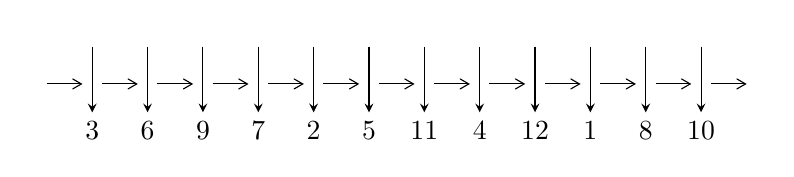
\begin{tikzpicture}[x=20pt, y=17pt]
	% nodes
	\node (C0) at (0, 0) {};
	\node (C1) at (1, 0) {};
	\node (C1U) at (1, +1) {};
	\node (C1D) at (1, -1) {3};

	\node (C2) at (2, 0) {};
	\node (C2U) at (2, +1) {};
	\node (C2D) at (2, -1) {6};

	\node (C3) at (3, 0) {};
	\node (C3U) at (3, +1) {};
	\node (C3D) at (3, -1) {9};

	\node (C4) at (4, 0) {};
	\node (C4U) at (4, +1) {};
	\node (C4D) at (4, -1) {7};

	\node (C5) at (5, 0) {};
	\node (C5U) at (5, +1) {};
	\node (C5D) at (5, -1) {2};

	\node (C6) at (6, 0) {};
	\node (C6U) at (6, +1) {};
	\node (C6D) at (6, -1) {5};

	\node (C7) at (7, 0) {};
	\node (C7U) at (7, +1) {};
	\node (C7D) at (7, -1) {11};

	\node (C8) at (8, 0) {};
	\node (C8U) at (8, +1) {};
	\node (C8D) at (8, -1) {4};

	\node (C9) at (9, 0) {};
	\node (C9U) at (9, +1) {};
	\node (C9D) at (9, -1) {12};

	\node (C10) at (10, 0) {};
	\node (C10U) at (10, +1) {};
	\node (C10D) at (10, -1) {1};

	\node (C11) at (11, 0) {};
	\node (C11U) at (11, +1) {};
	\node (C11D) at (11, -1) {8};

	\node (C12) at (12, 0) {};
	\node (C12U) at (12, +1) {};
	\node (C12D) at (12, -1) {10};
	\node (C13) at (13, 0) {};

	% arrows
	\draw[->,>={angle 60}]
	(C0) edge (C1) (C1) edge (C2) (C2) edge (C3) (C3) edge (C4) (C4) edge (C5) (C5) edge (C6) (C6) edge (C7) (C7) edge (C8) (C8) edge (C9) (C9) edge (C10) (C10) edge (C11) (C11) edge (C12) (C12) edge (C13) ;	\draw[->,>=stealth]
	(C1U) edge (C1D) (C2U) edge (C2D) (C3U) edge (C3D) (C4U) edge (C4D) (C5U) edge (C5D) (C6U) edge (C6D) (C7U) edge (C7D) (C8U) edge (C8D) (C9U) edge (C9D) (C10U) edge (C10D) (C11U) edge (C11D) (C12U) edge (C12D) ;
	\end{tikzpicture} \\
\hhline{~~} \\& 
\textbf{Solving Sequence} \\ \cline{2-2} 
 &
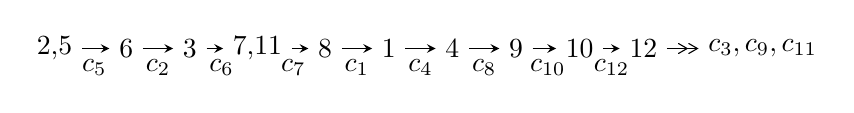
\begin{tikzpicture}[x=23pt, y=7pt]
	% node
	\node (A0) at (-1/8, 0) {2,5};
	\node (A1) at (1, 0) {6};
	\node (A2) at (2, 0) {3};
	\node (A3) at (49/16, 0) {7,11};
	\node (A4) at (33/8, 0) {8};
	\node (A5) at (41/8, 0) {1};
	\node (A6) at (49/8, 0) {4};
	\node (A7) at (57/8, 0) {9};
	\node (A8) at (65/8, 0) {10};
	\node (A9) at (73/8, 0) {12};
	\node (C1) at (1/2, -1) {$c_{5}$};
	\node (C2) at (3/2, -1) {$c_{2}$};
	\node (C3) at (5/2, -1) {$c_{6}$};
	\node (C4) at (29/8, -1) {$c_{7}$};
	\node (C5) at (37/8, -1) {$c_{1}$};
	\node (C6) at (45/8, -1) {$c_{4}$};
	\node (C7) at (53/8, -1) {$c_{8}$};
	\node (C8) at (61/8, -1) {$c_{10}$};
	\node (C9) at (69/8, -1) {$c_{12}$};
	\node (A10) at (11, 0) {$c_{3},c_{9},c_{11}$};

	% edge
	\draw[->,>=stealth]	
	(A0) edge (A1) (A1) edge (A2) (A2) edge (A3) (A3) edge (A4) (A4) edge (A5) (A5) edge (A6) (A6) edge (A7) (A7) edge (A8) (A8) edge (A9) ;
	\draw[->>,>={angle 60}]	
	(A9) edge (A10);
\end{tikzpicture} \\ 

\end{tabular} \\

\footnotetext{
The image of knot diagram is generated by the software ``\textbf{Draw programme}" developed by Andrew Bartholomew(\url{http://www.layer8.co.uk/maths/draw/index.htm\#Running-draw}), where we modified some parts for our purpose(\url{https://github.com/CATsTAILs/LinksPainter}).
}\phantom \\ \newline 
\centering \textbf{Ideals for irreducible components\footnotemark of $X_{\text{par}}$} 
 
\begin{align*}
I^u_{1}&=\langle 
-9.85235\times10^{24} u^{79}-2.72115\times10^{25} u^{78}+\cdots+9.93119\times10^{23} b-7.91401\times10^{24},\\
\phantom{I^u_{1}}&\phantom{= \langle  }-6.33480\times10^{24} u^{79}-2.53760\times10^{25} u^{78}+\cdots+1.98624\times10^{24} a-1.64622\times10^{25},\;u^{80}+4 u^{79}+\cdots+6 u+1\rangle \\
I^u_{2}&=\langle 
u^4- u^2+b- u+2,\;2 u^4+u^3+a-2 u+2,\;u^5+u^4- u^2+u+1\rangle \\
I^u_{3}&=\langle 
u^2+b,\;-2 u^2 a+a^2+a u-2 u^2+a+2 u-1,\;u^3- u^2+1\rangle \\
\\
\end{align*}
\raggedright * 3 irreducible components of $\dim_{\mathbb{C}}=0$, with total 91 representations.\\
\footnotetext{All coefficients of polynomials are rational numbers. But the coefficients are sometimes approximated in decimal forms when there is not enough margin.}
\newpage
\renewcommand{\arraystretch}{1}
\centering \section*{I. $I^u_{1}= \langle -9.85\times10^{24} u^{79}-2.72\times10^{25} u^{78}+\cdots+9.93\times10^{23} b-7.91\times10^{24},\;-6.33\times10^{24} u^{79}-2.54\times10^{25} u^{78}+\cdots+1.99\times10^{24} a-1.65\times10^{25},\;u^{80}+4 u^{79}+\cdots+6 u+1 \rangle$}
\flushleft \textbf{(i) Arc colorings}\\
\begin{tabular}{m{7pt} m{180pt} m{7pt} m{180pt} }
\flushright $a_{2}=$&$\begin{pmatrix}0\\u\end{pmatrix}$ \\
\flushright $a_{5}=$&$\begin{pmatrix}1\\0\end{pmatrix}$ \\
\flushright $a_{6}=$&$\begin{pmatrix}1\\u^2\end{pmatrix}$ \\
\flushright $a_{3}=$&$\begin{pmatrix}- u\\- u^3+u\end{pmatrix}$ \\
\flushright $a_{7}=$&$\begin{pmatrix}- u^2+1\\u^2\end{pmatrix}$ \\
\flushright $a_{11}=$&$\begin{pmatrix}3.18934 u^{79}+12.7759 u^{78}+\cdots+47.5761 u+8.28813\\9.92061 u^{79}+27.4001 u^{78}+\cdots+40.9951 u+7.96884\end{pmatrix}$ \\
\flushright $a_{8}=$&$\begin{pmatrix}7.35876 u^{79}+21.6854 u^{78}+\cdots+23.9027 u+7.03413\\-0.876176 u^{79}+2.07029 u^{78}+\cdots+16.0513 u+4.25701\end{pmatrix}$ \\
\flushright $a_{1}=$&$\begin{pmatrix}u^3\\u^5- u^3+u\end{pmatrix}$ \\
\flushright $a_{4}=$&$\begin{pmatrix}u^4- u^2+1\\- u^4\end{pmatrix}$ \\
\flushright $a_{9}=$&$\begin{pmatrix}-1.44610 u^{79}-3.25664 u^{78}+\cdots-0.0887997 u+2.46775\\3.89301 u^{79}+9.15127 u^{78}+\cdots+9.76680 u+2.44691\end{pmatrix}$ \\
\flushright $a_{10}=$&$\begin{pmatrix}3.89399 u^{79}+14.3516 u^{78}+\cdots+46.8184 u+7.87170\\8.12729 u^{79}+22.9501 u^{78}+\cdots+35.1348 u+6.87334\end{pmatrix}$ \\
\flushright $a_{12}=$&$\begin{pmatrix}7.21937 u^{79}+24.5178 u^{78}+\cdots+58.4840 u+11.4296\\7.78413 u^{79}+24.6495 u^{78}+\cdots+45.8212 u+9.60214\end{pmatrix}$\\&\end{tabular}
\flushleft \textbf{(ii) Obstruction class $= -1$}\\~\\
\flushleft \textbf{(iii) Cusp Shapes $= \frac{225344555042881471562867245}{993119401398295715683309} u^{79}+\frac{1486568910759558927791433433}{1986238802796591431366618} u^{78}+\cdots+\frac{2947932581577874658457472291}{1986238802796591431366618} u+\frac{619487791938232455082216191}{1986238802796591431366618}$}\\~\\
\newpage\renewcommand{\arraystretch}{1}
\flushleft \textbf{(iv) u-Polynomials at the component}\newline \\
\begin{tabular}{m{50pt}|m{274pt}}
Crossings & \hspace{64pt}u-Polynomials at each crossing \\
\hline $$\begin{aligned}c_{1},c_{4},c_{6}\end{aligned}$$&$\begin{aligned}
&u^{80}+20 u^{79}+\cdots+42 u+1
\end{aligned}$\\
\hline $$\begin{aligned}c_{2},c_{5}\end{aligned}$$&$\begin{aligned}
&u^{80}+4 u^{79}+\cdots+6 u+1
\end{aligned}$\\
\hline $$\begin{aligned}c_{3},c_{8}\end{aligned}$$&$\begin{aligned}
&u^{80}-2 u^{79}+\cdots+160 u-64
\end{aligned}$\\
\hline $$\begin{aligned}c_{7},c_{11}\end{aligned}$$&$\begin{aligned}
&u^{80}+4 u^{79}+\cdots-128 u-32
\end{aligned}$\\
\hline $$\begin{aligned}c_{9},c_{10},c_{12}\end{aligned}$$&$\begin{aligned}
&u^{80}-9 u^{79}+\cdots+27 u+1
\end{aligned}$\\
\hline
\end{tabular}\\~\\
\newpage\renewcommand{\arraystretch}{1}
\flushleft \textbf{(v) Riley Polynomials at the component}\newline \\
\begin{tabular}{m{50pt}|m{274pt}}
Crossings & \hspace{64pt}Riley Polynomials at each crossing \\
\hline $$\begin{aligned}c_{1},c_{4},c_{6}\end{aligned}$$&$\begin{aligned}
&y^{80}+84 y^{79}+\cdots-682 y+1
\end{aligned}$\\
\hline $$\begin{aligned}c_{2},c_{5}\end{aligned}$$&$\begin{aligned}
&y^{80}-20 y^{79}+\cdots-42 y+1
\end{aligned}$\\
\hline $$\begin{aligned}c_{3},c_{8}\end{aligned}$$&$\begin{aligned}
&y^{80}+42 y^{79}+\cdots-5120 y+4096
\end{aligned}$\\
\hline $$\begin{aligned}c_{7},c_{11}\end{aligned}$$&$\begin{aligned}
&y^{80}-42 y^{79}+\cdots-66048 y+1024
\end{aligned}$\\
\hline $$\begin{aligned}c_{9},c_{10},c_{12}\end{aligned}$$&$\begin{aligned}
&y^{80}-75 y^{79}+\cdots-213 y+1
\end{aligned}$\\
\hline
\end{tabular}\\~\\
\newpage\flushleft \textbf{(vi) Complex Volumes and Cusp Shapes}
$$\begin{array}{c|c|c}  
\text{Solutions to }I^u_{1}& \I (\text{vol} + \sqrt{-1}CS) & \text{Cusp shape}\\
 \hline 
\begin{aligned}
u &= \phantom{-}0.937313 + 0.347751 I \\
a &= \phantom{-}0.174266 - 0.787568 I \\
b &= -0.727576 + 0.727455 I\end{aligned}
 & -3.33822 - 4.82117 I & \phantom{-0.000000 } 0 \\ \hline\begin{aligned}
u &= \phantom{-}0.937313 - 0.347751 I \\
a &= \phantom{-}0.174266 + 0.787568 I \\
b &= -0.727576 - 0.727455 I\end{aligned}
 & -3.33822 + 4.82117 I & \phantom{-0.000000 } 0 \\ \hline\begin{aligned}
u &= \phantom{-}0.582846 + 0.818388 I \\
a &= -0.672268 + 0.203176 I \\
b &= -0.086980 - 0.893421 I\end{aligned}
 & -1.26973 - 4.01147 I & \phantom{-0.000000 } 0 \\ \hline\begin{aligned}
u &= \phantom{-}0.582846 - 0.818388 I \\
a &= -0.672268 - 0.203176 I \\
b &= -0.086980 + 0.893421 I\end{aligned}
 & -1.26973 + 4.01147 I & \phantom{-0.000000 } 0 \\ \hline\begin{aligned}
u &= \phantom{-}0.845099 + 0.506123 I \\
a &= -0.017809 + 0.337413 I \\
b &= \phantom{-}0.369387 - 0.227156 I\end{aligned}
 & \phantom{-}1.73618 - 2.77244 I & \phantom{-0.000000 } 0 \\ \hline\begin{aligned}
u &= \phantom{-}0.845099 - 0.506123 I \\
a &= -0.017809 - 0.337413 I \\
b &= \phantom{-}0.369387 + 0.227156 I\end{aligned}
 & \phantom{-}1.73618 + 2.77244 I & \phantom{-0.000000 } 0 \\ \hline\begin{aligned}
u &= -0.950543 + 0.403879 I \\
a &= \phantom{-}0.090000 - 0.577227 I \\
b &= -0.64347 - 1.42153 I\end{aligned}
 & -8.56535 + 4.83425 I & \phantom{-0.000000 } 0 \\ \hline\begin{aligned}
u &= -0.950543 - 0.403879 I \\
a &= \phantom{-}0.090000 + 0.577227 I \\
b &= -0.64347 + 1.42153 I\end{aligned}
 & -8.56535 - 4.83425 I & \phantom{-0.000000 } 0 \\ \hline\begin{aligned}
u &= -0.959530 + 0.120935 I \\
a &= -0.838995 - 0.755294 I \\
b &= -0.656494 + 0.002059 I\end{aligned}
 & -2.04664 - 1.46066 I & \phantom{-0.000000 } 0 \\ \hline\begin{aligned}
u &= -0.959530 - 0.120935 I \\
a &= -0.838995 + 0.755294 I \\
b &= -0.656494 - 0.002059 I\end{aligned}
 & -2.04664 + 1.46066 I & \phantom{-0.000000 } 0\\
 \hline 
 \end{array}$$\newpage$$\begin{array}{c|c|c}  
\text{Solutions to }I^u_{1}& \I (\text{vol} + \sqrt{-1}CS) & \text{Cusp shape}\\
 \hline 
\begin{aligned}
u &= \phantom{-}0.975562 + 0.382659 I \\
a &= -0.471936 + 0.931640 I \\
b &= -1.112520 + 0.332535 I\end{aligned}
 & -0.55792 - 7.07014 I & \phantom{-0.000000 } 0 \\ \hline\begin{aligned}
u &= \phantom{-}0.975562 - 0.382659 I \\
a &= -0.471936 - 0.931640 I \\
b &= -1.112520 - 0.332535 I\end{aligned}
 & -0.55792 + 7.07014 I & \phantom{-0.000000 } 0 \\ \hline\begin{aligned}
u &= \phantom{-}0.870682 + 0.332652 I \\
a &= \phantom{-}1.25916 - 1.20100 I \\
b &= \phantom{-}0.603918 + 0.379611 I\end{aligned}
 & -2.02857 - 2.17557 I & \phantom{-0.000000 } 0 \\ \hline\begin{aligned}
u &= \phantom{-}0.870682 - 0.332652 I \\
a &= \phantom{-}1.25916 + 1.20100 I \\
b &= \phantom{-}0.603918 - 0.379611 I\end{aligned}
 & -2.02857 + 2.17557 I & \phantom{-0.000000 } 0 \\ \hline\begin{aligned}
u &= -0.904570 + 0.199072 I \\
a &= \phantom{-}0.152725 - 0.178138 I \\
b &= \phantom{-}1.40879 + 0.86692 I\end{aligned}
 & -4.19881 + 0.29220 I & \phantom{-0.000000 } 0 \\ \hline\begin{aligned}
u &= -0.904570 - 0.199072 I \\
a &= \phantom{-}0.152725 + 0.178138 I \\
b &= \phantom{-}1.40879 - 0.86692 I\end{aligned}
 & -4.19881 - 0.29220 I & \phantom{-0.000000 } 0 \\ \hline\begin{aligned}
u &= -1.069250 + 0.146998 I \\
a &= \phantom{-}0.899094 + 0.683161 I \\
b &= -0.0510110 - 0.0498696 I\end{aligned}
 & -7.63820 - 4.53013 I & \phantom{-0.000000 } 0 \\ \hline\begin{aligned}
u &= -1.069250 - 0.146998 I \\
a &= \phantom{-}0.899094 - 0.683161 I \\
b &= -0.0510110 + 0.0498696 I\end{aligned}
 & -7.63820 + 4.53013 I & \phantom{-0.000000 } 0 \\ \hline\begin{aligned}
u &= -0.853249 + 0.283826 I \\
a &= \phantom{-}0.382918 + 1.152640 I \\
b &= \phantom{-}0.939067 + 0.906091 I\end{aligned}
 & -2.31119 + 2.17762 I & \phantom{-0.000000 } 0 \\ \hline\begin{aligned}
u &= -0.853249 - 0.283826 I \\
a &= \phantom{-}0.382918 - 1.152640 I \\
b &= \phantom{-}0.939067 - 0.906091 I\end{aligned}
 & -2.31119 - 2.17762 I & \phantom{-0.000000 } 0\\
 \hline 
 \end{array}$$\newpage$$\begin{array}{c|c|c}  
\text{Solutions to }I^u_{1}& \I (\text{vol} + \sqrt{-1}CS) & \text{Cusp shape}\\
 \hline 
\begin{aligned}
u &= \phantom{-}1.047550 + 0.374433 I \\
a &= \phantom{-}0.269786 - 0.393377 I \\
b &= \phantom{-}1.006870 - 0.937317 I\end{aligned}
 & -6.26460 - 11.20980 I & \phantom{-0.000000 } 0 \\ \hline\begin{aligned}
u &= \phantom{-}1.047550 - 0.374433 I \\
a &= \phantom{-}0.269786 + 0.393377 I \\
b &= \phantom{-}1.006870 + 0.937317 I\end{aligned}
 & -6.26460 + 11.20980 I & \phantom{-0.000000 } 0 \\ \hline\begin{aligned}
u &= \phantom{-}0.882220 + 0.717129 I \\
a &= -0.443888 + 1.246120 I \\
b &= -0.226602 - 0.774802 I\end{aligned}
 & \phantom{-}2.32601 - 2.74241 I & \phantom{-0.000000 } 0 \\ \hline\begin{aligned}
u &= \phantom{-}0.882220 - 0.717129 I \\
a &= -0.443888 - 1.246120 I \\
b &= -0.226602 + 0.774802 I\end{aligned}
 & \phantom{-}2.32601 + 2.74241 I & \phantom{-0.000000 } 0 \\ \hline\begin{aligned}
u &= \phantom{-}0.848871 + 0.109256 I \\
a &= -1.96581 + 0.51451 I \\
b &= \phantom{-}0.377107 - 0.195551 I\end{aligned}
 & -10.28610 - 0.13892 I & -24.9438 + 9.7256 I \\ \hline\begin{aligned}
u &= \phantom{-}0.848871 - 0.109256 I \\
a &= -1.96581 - 0.51451 I \\
b &= \phantom{-}0.377107 + 0.195551 I\end{aligned}
 & -10.28610 + 0.13892 I & -24.9438 - 9.7256 I \\ \hline\begin{aligned}
u &= \phantom{-}0.859887 + 0.789823 I \\
a &= \phantom{-}2.69951 + 2.32641 I \\
b &= -3.15862 + 0.26803 I\end{aligned}
 & \phantom{-}1.64882 - 2.07054 I & \phantom{-0.000000 } 0 \\ \hline\begin{aligned}
u &= \phantom{-}0.859887 - 0.789823 I \\
a &= \phantom{-}2.69951 - 2.32641 I \\
b &= -3.15862 - 0.26803 I\end{aligned}
 & \phantom{-}1.64882 + 2.07054 I & \phantom{-0.000000 } 0 \\ \hline\begin{aligned}
u &= -0.892015 + 0.791150 I \\
a &= \phantom{-}0.598424 + 0.150430 I \\
b &= \phantom{-}0.240714 - 1.363070 I\end{aligned}
 & -5.15784 + 2.97447 I & \phantom{-0.000000 } 0 \\ \hline\begin{aligned}
u &= -0.892015 - 0.791150 I \\
a &= \phantom{-}0.598424 - 0.150430 I \\
b &= \phantom{-}0.240714 + 1.363070 I\end{aligned}
 & -5.15784 - 2.97447 I & \phantom{-0.000000 } 0\\
 \hline 
 \end{array}$$\newpage$$\begin{array}{c|c|c}  
\text{Solutions to }I^u_{1}& \I (\text{vol} + \sqrt{-1}CS) & \text{Cusp shape}\\
 \hline 
\begin{aligned}
u &= -0.836397 + 0.864338 I \\
a &= -2.07623 + 0.93166 I \\
b &= \phantom{-}2.19378 + 1.00704 I\end{aligned}
 & \phantom{-}4.36446 - 2.41660 I & \phantom{-0.000000 } 0 \\ \hline\begin{aligned}
u &= -0.836397 - 0.864338 I \\
a &= -2.07623 - 0.93166 I \\
b &= \phantom{-}2.19378 - 1.00704 I\end{aligned}
 & \phantom{-}4.36446 + 2.41660 I & \phantom{-0.000000 } 0 \\ \hline\begin{aligned}
u &= \phantom{-}0.865180 + 0.835627 I \\
a &= \phantom{-}1.50909 + 1.74688 I \\
b &= -2.39004 - 0.66512 I\end{aligned}
 & \phantom{-}4.48911 - 0.87143 I & \phantom{-0.000000 } 0 \\ \hline\begin{aligned}
u &= \phantom{-}0.865180 - 0.835627 I \\
a &= \phantom{-}1.50909 - 1.74688 I \\
b &= -2.39004 + 0.66512 I\end{aligned}
 & \phantom{-}4.48911 + 0.87143 I & \phantom{-0.000000 } 0 \\ \hline\begin{aligned}
u &= \phantom{-}0.917805 + 0.779835 I \\
a &= -2.54765 - 1.79888 I \\
b &= \phantom{-}3.28237 - 0.10616 I\end{aligned}
 & \phantom{-}1.47178 - 3.83910 I & \phantom{-0.000000 } 0 \\ \hline\begin{aligned}
u &= \phantom{-}0.917805 - 0.779835 I \\
a &= -2.54765 + 1.79888 I \\
b &= \phantom{-}3.28237 + 0.10616 I\end{aligned}
 & \phantom{-}1.47178 + 3.83910 I & \phantom{-0.000000 } 0 \\ \hline\begin{aligned}
u &= \phantom{-}0.494296 + 0.619420 I \\
a &= -0.118161 + 0.445938 I \\
b &= \phantom{-}0.050487 + 0.469304 I\end{aligned}
 & \phantom{-}2.81647 - 1.39098 I & -4.65333 + 3.39574 I \\ \hline\begin{aligned}
u &= \phantom{-}0.494296 - 0.619420 I \\
a &= -0.118161 - 0.445938 I \\
b &= \phantom{-}0.050487 - 0.469304 I\end{aligned}
 & \phantom{-}2.81647 + 1.39098 I & -4.65333 - 3.39574 I \\ \hline\begin{aligned}
u &= -0.800901 + 0.904702 I \\
a &= \phantom{-}1.55800 - 1.78263 I \\
b &= -2.53254 + 0.77113 I\end{aligned}
 & \phantom{-}2.23380 - 9.78191 I & \phantom{-0.000000 } 0 \\ \hline\begin{aligned}
u &= -0.800901 - 0.904702 I \\
a &= \phantom{-}1.55800 + 1.78263 I \\
b &= -2.53254 - 0.77113 I\end{aligned}
 & \phantom{-}2.23380 + 9.78191 I & \phantom{-0.000000 } 0\\
 \hline 
 \end{array}$$\newpage$$\begin{array}{c|c|c}  
\text{Solutions to }I^u_{1}& \I (\text{vol} + \sqrt{-1}CS) & \text{Cusp shape}\\
 \hline 
\begin{aligned}
u &= -0.856330 + 0.854982 I \\
a &= \phantom{-}1.166280 - 0.386013 I \\
b &= -1.60157 + 0.16248 I\end{aligned}
 & \phantom{-}5.34443 + 0.79481 I & \phantom{-0.000000 } 0 \\ \hline\begin{aligned}
u &= -0.856330 - 0.854982 I \\
a &= \phantom{-}1.166280 + 0.386013 I \\
b &= -1.60157 - 0.16248 I\end{aligned}
 & \phantom{-}5.34443 - 0.79481 I & \phantom{-0.000000 } 0 \\ \hline\begin{aligned}
u &= -0.828964 + 0.884459 I \\
a &= -1.60651 + 1.16176 I \\
b &= \phantom{-}2.28569 - 0.38260 I\end{aligned}
 & \phantom{-}7.64873 - 4.89072 I & \phantom{-0.000000 } 0 \\ \hline\begin{aligned}
u &= -0.828964 - 0.884459 I \\
a &= -1.60651 - 1.16176 I \\
b &= \phantom{-}2.28569 + 0.38260 I\end{aligned}
 & \phantom{-}7.64873 + 4.89072 I & \phantom{-0.000000 } 0 \\ \hline\begin{aligned}
u &= \phantom{-}1.017270 + 0.661319 I \\
a &= -0.318473 + 0.115749 I \\
b &= -0.238056 - 0.984477 I\end{aligned}
 & -2.61888 - 1.46312 I & \phantom{-0.000000 } 0 \\ \hline\begin{aligned}
u &= \phantom{-}1.017270 - 0.661319 I \\
a &= -0.318473 - 0.115749 I \\
b &= -0.238056 + 0.984477 I\end{aligned}
 & -2.61888 + 1.46312 I & \phantom{-0.000000 } 0 \\ \hline\begin{aligned}
u &= \phantom{-}0.169440 + 0.760477 I \\
a &= \phantom{-}0.000302 + 0.920026 I \\
b &= -0.886187 - 0.066321 I\end{aligned}
 & -3.38617 + 7.21522 I & -11.57739 - 4.93181 I \\ \hline\begin{aligned}
u &= \phantom{-}0.169440 - 0.760477 I \\
a &= \phantom{-}0.000302 - 0.920026 I \\
b &= -0.886187 + 0.066321 I\end{aligned}
 & -3.38617 - 7.21522 I & -11.57739 + 4.93181 I \\ \hline\begin{aligned}
u &= \phantom{-}0.838303 + 0.889934 I \\
a &= -0.82802 - 2.20009 I \\
b &= \phantom{-}2.09293 + 1.43375 I\end{aligned}
 & -0.22327 + 2.37163 I & \phantom{-0.000000 } 0 \\ \hline\begin{aligned}
u &= \phantom{-}0.838303 - 0.889934 I \\
a &= -0.82802 + 2.20009 I \\
b &= \phantom{-}2.09293 - 1.43375 I\end{aligned}
 & -0.22327 - 2.37163 I & \phantom{-0.000000 } 0\\
 \hline 
 \end{array}$$\newpage$$\begin{array}{c|c|c}  
\text{Solutions to }I^u_{1}& \I (\text{vol} + \sqrt{-1}CS) & \text{Cusp shape}\\
 \hline 
\begin{aligned}
u &= \phantom{-}0.933131 + 0.813064 I \\
a &= -2.36608 - 1.04014 I \\
b &= \phantom{-}2.31780 - 1.05442 I\end{aligned}
 & \phantom{-}4.27708 - 5.28117 I & \phantom{-0.000000 } 0 \\ \hline\begin{aligned}
u &= \phantom{-}0.933131 - 0.813064 I \\
a &= -2.36608 + 1.04014 I \\
b &= \phantom{-}2.31780 + 1.05442 I\end{aligned}
 & \phantom{-}4.27708 + 5.28117 I & \phantom{-0.000000 } 0 \\ \hline\begin{aligned}
u &= -0.887481 + 0.879573 I \\
a &= \phantom{-}1.58106 - 0.65269 I \\
b &= -1.76830 - 0.70972 I\end{aligned}
 & \phantom{-}10.21390 + 1.20204 I & \phantom{-0.000000 } 0 \\ \hline\begin{aligned}
u &= -0.887481 - 0.879573 I \\
a &= \phantom{-}1.58106 + 0.65269 I \\
b &= -1.76830 + 0.70972 I\end{aligned}
 & \phantom{-}10.21390 - 1.20204 I & \phantom{-0.000000 } 0 \\ \hline\begin{aligned}
u &= -0.948192 + 0.820603 I \\
a &= -1.13552 + 1.28892 I \\
b &= \phantom{-}1.38937 + 0.40661 I\end{aligned}
 & \phantom{-}5.05593 + 5.43924 I & \phantom{-0.000000 } 0 \\ \hline\begin{aligned}
u &= -0.948192 - 0.820603 I \\
a &= -1.13552 - 1.28892 I \\
b &= \phantom{-}1.38937 - 0.40661 I\end{aligned}
 & \phantom{-}5.05593 - 5.43924 I & \phantom{-0.000000 } 0 \\ \hline\begin{aligned}
u &= -0.965009 + 0.816000 I \\
a &= \phantom{-}1.18309 - 1.63202 I \\
b &= -2.56538 + 0.59228 I\end{aligned}
 & \phantom{-}3.96142 + 8.66250 I & \phantom{-0.000000 } 0 \\ \hline\begin{aligned}
u &= -0.965009 - 0.816000 I \\
a &= \phantom{-}1.18309 + 1.63202 I \\
b &= -2.56538 - 0.59228 I\end{aligned}
 & \phantom{-}3.96142 - 8.66250 I & \phantom{-0.000000 } 0 \\ \hline\begin{aligned}
u &= -0.942925 + 0.856435 I \\
a &= -0.96892 + 1.24837 I \\
b &= \phantom{-}1.88035 - 0.35749 I\end{aligned}
 & \phantom{-}10.03880 + 5.22302 I & \phantom{-0.000000 } 0 \\ \hline\begin{aligned}
u &= -0.942925 - 0.856435 I \\
a &= -0.96892 - 1.24837 I \\
b &= \phantom{-}1.88035 + 0.35749 I\end{aligned}
 & \phantom{-}10.03880 - 5.22302 I & \phantom{-0.000000 } 0\\
 \hline 
 \end{array}$$\newpage$$\begin{array}{c|c|c}  
\text{Solutions to }I^u_{1}& \I (\text{vol} + \sqrt{-1}CS) & \text{Cusp shape}\\
 \hline 
\begin{aligned}
u &= -0.979592 + 0.822863 I \\
a &= \phantom{-}1.89112 - 1.38953 I \\
b &= -2.23000 - 0.70512 I\end{aligned}
 & \phantom{-}7.17373 + 11.21830 I & \phantom{-0.000000 } 0 \\ \hline\begin{aligned}
u &= -0.979592 - 0.822863 I \\
a &= \phantom{-}1.89112 + 1.38953 I \\
b &= -2.23000 + 0.70512 I\end{aligned}
 & \phantom{-}7.17373 - 11.21830 I & \phantom{-0.000000 } 0 \\ \hline\begin{aligned}
u &= \phantom{-}0.977444 + 0.830015 I \\
a &= \phantom{-}2.51218 + 0.28028 I \\
b &= -2.10646 + 1.76637 I\end{aligned}
 & -0.66511 - 8.73988 I & \phantom{-0.000000 } 0 \\ \hline\begin{aligned}
u &= \phantom{-}0.977444 - 0.830015 I \\
a &= \phantom{-}2.51218 - 0.28028 I \\
b &= -2.10646 - 1.76637 I\end{aligned}
 & -0.66511 + 8.73988 I & \phantom{-0.000000 } 0 \\ \hline\begin{aligned}
u &= -0.321779 + 0.632139 I \\
a &= \phantom{-}0.756357 + 0.960282 I \\
b &= \phantom{-}0.871646 - 0.585910 I\end{aligned}
 & -6.55850 - 1.01923 I & -15.1391 + 0. I\phantom{ +0.000000I} \\ \hline\begin{aligned}
u &= -0.321779 - 0.632139 I \\
a &= \phantom{-}0.756357 - 0.960282 I \\
b &= \phantom{-}0.871646 + 0.585910 I\end{aligned}
 & -6.55850 + 1.01923 I & -15.1391 + 0. I\phantom{ +0.000000I} \\ \hline\begin{aligned}
u &= -1.004210 + 0.817409 I \\
a &= -2.33088 + 1.12360 I \\
b &= \phantom{-}2.59048 + 1.17800 I\end{aligned}
 & \phantom{-}1.5910 + 16.1481 I & \phantom{-0.000000 } 0 \\ \hline\begin{aligned}
u &= -1.004210 - 0.817409 I \\
a &= -2.33088 - 1.12360 I \\
b &= \phantom{-}2.59048 - 1.17800 I\end{aligned}
 & \phantom{-}1.5910 - 16.1481 I & \phantom{-0.000000 } 0 \\ \hline\begin{aligned}
u &= -0.700562\phantom{ +0.000000I} \\
a &= -4.30574\phantom{ +0.000000I} \\
b &= -3.73829\phantom{ +0.000000I}\end{aligned}
 & -2.59838\phantom{ +0.000000I} & -119.010\phantom{ +0.000000I} \\ \hline\begin{aligned}
u &= \phantom{-}0.237042 + 0.644569 I \\
a &= -0.711917 - 0.474272 I \\
b &= \phantom{-}1.050580 - 0.217495 I\end{aligned}
 & \phantom{-}1.76492 + 3.34953 I & -6.94493 - 4.05394 I\\
 \hline 
 \end{array}$$\newpage$$\begin{array}{c|c|c}  
\text{Solutions to }I^u_{1}& \I (\text{vol} + \sqrt{-1}CS) & \text{Cusp shape}\\
 \hline 
\begin{aligned}
u &= \phantom{-}0.237042 - 0.644569 I \\
a &= -0.711917 + 0.474272 I \\
b &= \phantom{-}1.050580 + 0.217495 I\end{aligned}
 & \phantom{-}1.76492 - 3.34953 I & -6.94493 + 4.05394 I \\ \hline\begin{aligned}
u &= -0.941907 + 0.920353 I \\
a &= -0.680992 - 0.844842 I \\
b &= \phantom{-}0.006272 + 1.215720 I\end{aligned}
 & \phantom{-}8.88798 + 3.38254 I & \phantom{-0.000000 } 0 \\ \hline\begin{aligned}
u &= -0.941907 - 0.920353 I \\
a &= -0.680992 + 0.844842 I \\
b &= \phantom{-}0.006272 - 1.215720 I\end{aligned}
 & \phantom{-}8.88798 - 3.38254 I & \phantom{-0.000000 } 0 \\ \hline\begin{aligned}
u &= -0.578820\phantom{ +0.000000I} \\
a &= -0.441740\phantom{ +0.000000I} \\
b &= -0.634881\phantom{ +0.000000I}\end{aligned}
 & -0.838544\phantom{ +0.000000I} & -11.3510\phantom{ +0.000000I} \\ \hline\begin{aligned}
u &= \phantom{-}0.406147 + 0.408093 I \\
a &= \phantom{-}1.80938 - 0.53475 I \\
b &= -0.854606 + 0.774894 I\end{aligned}
 & -0.571047 - 0.765230 I & -10.03702 + 1.06541 I \\ \hline\begin{aligned}
u &= \phantom{-}0.406147 - 0.408093 I \\
a &= \phantom{-}1.80938 + 0.53475 I \\
b &= -0.854606 - 0.774894 I\end{aligned}
 & -0.571047 + 0.765230 I & -10.03702 - 1.06541 I \\ \hline\begin{aligned}
u &= \phantom{-}0.215457 + 0.521353 I \\
a &= \phantom{-}0.91607 - 1.54710 I \\
b &= -0.199480 - 0.311181 I\end{aligned}
 & -1.18117 + 1.56184 I & -9.13121 - 0.95837 I \\ \hline\begin{aligned}
u &= \phantom{-}0.215457 - 0.521353 I \\
a &= \phantom{-}0.91607 + 1.54710 I \\
b &= -0.199480 + 0.311181 I\end{aligned}
 & -1.18117 - 1.56184 I & -9.13121 + 0.95837 I \\ \hline\begin{aligned}
u &= -0.482222\phantom{ +0.000000I} \\
a &= -0.713720\phantom{ +0.000000I} \\
b &= -0.780848\phantom{ +0.000000I}\end{aligned}
 & -0.843561\phantom{ +0.000000I} & -10.4350\phantom{ +0.000000I} \\ \hline\begin{aligned}
u &= -0.195815\phantom{ +0.000000I} \\
a &= -2.15633\phantom{ +0.000000I} \\
b &= -0.689441\phantom{ +0.000000I}\end{aligned}
 & -0.820251\phantom{ +0.000000I} & -11.7060\phantom{ +0.000000I}\\
 \hline 
 \end{array}$$\newpage\newpage\renewcommand{\arraystretch}{1}
\centering \section*{II. $I^u_{2}= \langle u^4- u^2+b- u+2,\;2 u^4+u^3+a-2 u+2,\;u^5+u^4- u^2+u+1 \rangle$}
\flushleft \textbf{(i) Arc colorings}\\
\begin{tabular}{m{7pt} m{180pt} m{7pt} m{180pt} }
\flushright $a_{2}=$&$\begin{pmatrix}0\\u\end{pmatrix}$ \\
\flushright $a_{5}=$&$\begin{pmatrix}1\\0\end{pmatrix}$ \\
\flushright $a_{6}=$&$\begin{pmatrix}1\\u^2\end{pmatrix}$ \\
\flushright $a_{3}=$&$\begin{pmatrix}- u\\- u^3+u\end{pmatrix}$ \\
\flushright $a_{7}=$&$\begin{pmatrix}- u^2+1\\u^2\end{pmatrix}$ \\
\flushright $a_{11}=$&$\begin{pmatrix}-2 u^4- u^3+2 u-2\\- u^4+u^2+u-2\end{pmatrix}$ \\
\flushright $a_{8}=$&$\begin{pmatrix}- u^2+1\\u^2\end{pmatrix}$ \\
\flushright $a_{1}=$&$\begin{pmatrix}u^3\\- u^4- u^3+u^2-1\end{pmatrix}$ \\
\flushright $a_{4}=$&$\begin{pmatrix}u^4- u^2+1\\- u^4\end{pmatrix}$ \\
\flushright $a_{9}=$&$\begin{pmatrix}- u^3\\u^4+u^3- u^2+1\end{pmatrix}$ \\
\flushright $a_{10}=$&$\begin{pmatrix}-2 u^4-2 u^3+2 u-2\\u^3+u-1\end{pmatrix}$ \\
\flushright $a_{12}=$&$\begin{pmatrix}-2 u^4- u^3+2 u-2\\- u^4+u^2+u-2\end{pmatrix}$\\&\end{tabular}
\flushleft \textbf{(ii) Obstruction class $= 1$}\\~\\
\flushleft \textbf{(iii) Cusp Shapes $= 10 u^4+7 u^3+u^2-10 u+7$}\\~\\
\newpage\renewcommand{\arraystretch}{1}
\flushleft \textbf{(iv) u-Polynomials at the component}\newline \\
\begin{tabular}{m{50pt}|m{274pt}}
Crossings & \hspace{64pt}u-Polynomials at each crossing \\
\hline $$\begin{aligned}c_{1},c_{3},c_{4}\end{aligned}$$&$\begin{aligned}
&u^5- u^4+4 u^3-3 u^2+3 u-1
\end{aligned}$\\
\hline $$\begin{aligned}c_{2}\end{aligned}$$&$\begin{aligned}
&u^5- u^4+u^2+u-1
\end{aligned}$\\
\hline $$\begin{aligned}c_{5}\end{aligned}$$&$\begin{aligned}
&u^5+u^4- u^2+u+1
\end{aligned}$\\
\hline $$\begin{aligned}c_{6},c_{8}\end{aligned}$$&$\begin{aligned}
&u^5+u^4+4 u^3+3 u^2+3 u+1
\end{aligned}$\\
\hline $$\begin{aligned}c_{7},c_{11}\end{aligned}$$&$\begin{aligned}
&u^5
\end{aligned}$\\
\hline $$\begin{aligned}c_{9},c_{10}\end{aligned}$$&$\begin{aligned}
&(u-1)^5
\end{aligned}$\\
\hline $$\begin{aligned}c_{12}\end{aligned}$$&$\begin{aligned}
&(u+1)^5
\end{aligned}$\\
\hline
\end{tabular}\\~\\
\newpage\renewcommand{\arraystretch}{1}
\flushleft \textbf{(v) Riley Polynomials at the component}\newline \\
\begin{tabular}{m{50pt}|m{274pt}}
Crossings & \hspace{64pt}Riley Polynomials at each crossing \\
\hline $$\begin{aligned}c_{1},c_{3},c_{4}\\c_{6},c_{8}\end{aligned}$$&$\begin{aligned}
&y^5+7 y^4+16 y^3+13 y^2+3 y-1
\end{aligned}$\\
\hline $$\begin{aligned}c_{2},c_{5}\end{aligned}$$&$\begin{aligned}
&y^5- y^4+4 y^3-3 y^2+3 y-1
\end{aligned}$\\
\hline $$\begin{aligned}c_{7},c_{11}\end{aligned}$$&$\begin{aligned}
&y^5
\end{aligned}$\\
\hline $$\begin{aligned}c_{9},c_{10},c_{12}\end{aligned}$$&$\begin{aligned}
&(y-1)^5
\end{aligned}$\\
\hline
\end{tabular}\\~\\
\newpage\flushleft \textbf{(vi) Complex Volumes and Cusp Shapes}
$$\begin{array}{c|c|c}  
\text{Solutions to }I^u_{2}& \I (\text{vol} + \sqrt{-1}CS) & \text{Cusp shape}\\
 \hline 
\begin{aligned}
u &= \phantom{-}0.758138 + 0.584034 I \\
a &= \phantom{-}1.315520 - 0.467517 I \\
b &= -0.278580 + 1.055720 I\end{aligned}
 & \phantom{-}0.17487 - 2.21397 I & -10.02401 + 4.83884 I \\ \hline\begin{aligned}
u &= \phantom{-}0.758138 - 0.584034 I \\
a &= \phantom{-}1.315520 + 0.467517 I \\
b &= -0.278580 - 1.055720 I\end{aligned}
 & \phantom{-}0.17487 + 2.21397 I & -10.02401 - 4.83884 I \\ \hline\begin{aligned}
u &= -0.935538 + 0.903908 I \\
a &= \phantom{-}0.368676 + 0.566573 I \\
b &= -0.020316 - 0.590570 I\end{aligned}
 & \phantom{-}9.31336 + 3.33174 I & -1.83654 - 1.25445 I \\ \hline\begin{aligned}
u &= -0.935538 - 0.903908 I \\
a &= \phantom{-}0.368676 - 0.566573 I \\
b &= -0.020316 + 0.590570 I\end{aligned}
 & \phantom{-}9.31336 - 3.33174 I & -1.83654 + 1.25445 I \\ \hline\begin{aligned}
u &= -0.645200\phantom{ +0.000000I} \\
a &= -3.36840\phantom{ +0.000000I} \\
b &= -2.40221\phantom{ +0.000000I}\end{aligned}
 & -2.52712\phantom{ +0.000000I} & \phantom{-}13.7210\phantom{ +0.000000I}\\
 \hline 
 \end{array}$$\newpage\newpage\renewcommand{\arraystretch}{1}
\centering \section*{III. $I^u_{3}= \langle u^2+b,\;-2 u^2 a+a^2+a u-2 u^2+a+2 u-1,\;u^3- u^2+1 \rangle$}
\flushleft \textbf{(i) Arc colorings}\\
\begin{tabular}{m{7pt} m{180pt} m{7pt} m{180pt} }
\flushright $a_{2}=$&$\begin{pmatrix}0\\u\end{pmatrix}$ \\
\flushright $a_{5}=$&$\begin{pmatrix}1\\0\end{pmatrix}$ \\
\flushright $a_{6}=$&$\begin{pmatrix}1\\u^2\end{pmatrix}$ \\
\flushright $a_{3}=$&$\begin{pmatrix}- u\\- u^2+u+1\end{pmatrix}$ \\
\flushright $a_{7}=$&$\begin{pmatrix}- u^2+1\\u^2\end{pmatrix}$ \\
\flushright $a_{11}=$&$\begin{pmatrix}a\\- u^2\end{pmatrix}$ \\
\flushright $a_{8}=$&$\begin{pmatrix}a u-2 u^2+2 u+1\\u^2 a- a u+3 u^2- a-1\end{pmatrix}$ \\
\flushright $a_{1}=$&$\begin{pmatrix}u^2-1\\- u^2\end{pmatrix}$ \\
\flushright $a_{4}=$&$\begin{pmatrix}- u\\- u^2+u+1\end{pmatrix}$ \\
\flushright $a_{9}=$&$\begin{pmatrix}a u-2 u^2+2 u+1\\u^2 a- a u+3 u^2- a-1\end{pmatrix}$ \\
\flushright $a_{10}=$&$\begin{pmatrix}- a u+2 u^2- u-2\\- u^2 a+a u-3 u^2+a+1\end{pmatrix}$ \\
\flushright $a_{12}=$&$\begin{pmatrix}2 a u-3 u^2+a+3 u+2\\2 u^2 a-2 a u+4 u^2-2 a-2\end{pmatrix}$\\&\end{tabular}
\flushleft \textbf{(ii) Obstruction class $= 1$}\\~\\
\flushleft \textbf{(iii) Cusp Shapes $= 3 u^2 a+4 u^2+3 a-2 u-15$}\\~\\
\newpage\renewcommand{\arraystretch}{1}
\flushleft \textbf{(iv) u-Polynomials at the component}\newline \\
\begin{tabular}{m{50pt}|m{274pt}}
Crossings & \hspace{64pt}u-Polynomials at each crossing \\
\hline $$\begin{aligned}c_{1},c_{4}\end{aligned}$$&$\begin{aligned}
&(u^3- u^2+2 u-1)^2
\end{aligned}$\\
\hline $$\begin{aligned}c_{2}\end{aligned}$$&$\begin{aligned}
&(u^3+u^2-1)^2
\end{aligned}$\\
\hline $$\begin{aligned}c_{3},c_{8}\end{aligned}$$&$\begin{aligned}
&u^6
\end{aligned}$\\
\hline $$\begin{aligned}c_{5}\end{aligned}$$&$\begin{aligned}
&(u^3- u^2+1)^2
\end{aligned}$\\
\hline $$\begin{aligned}c_{6}\end{aligned}$$&$\begin{aligned}
&(u^3+u^2+2 u+1)^2
\end{aligned}$\\
\hline $$\begin{aligned}c_{7},c_{9},c_{10}\end{aligned}$$&$\begin{aligned}
&(u^2+u-1)^3
\end{aligned}$\\
\hline $$\begin{aligned}c_{11},c_{12}\end{aligned}$$&$\begin{aligned}
&(u^2- u-1)^3
\end{aligned}$\\
\hline
\end{tabular}\\~\\
\newpage\renewcommand{\arraystretch}{1}
\flushleft \textbf{(v) Riley Polynomials at the component}\newline \\
\begin{tabular}{m{50pt}|m{274pt}}
Crossings & \hspace{64pt}Riley Polynomials at each crossing \\
\hline $$\begin{aligned}c_{1},c_{4},c_{6}\end{aligned}$$&$\begin{aligned}
&(y^3+3 y^2+2 y-1)^2
\end{aligned}$\\
\hline $$\begin{aligned}c_{2},c_{5}\end{aligned}$$&$\begin{aligned}
&(y^3- y^2+2 y-1)^2
\end{aligned}$\\
\hline $$\begin{aligned}c_{3},c_{8}\end{aligned}$$&$\begin{aligned}
&y^6
\end{aligned}$\\
\hline $$\begin{aligned}c_{7},c_{9},c_{10}\\c_{11},c_{12}\end{aligned}$$&$\begin{aligned}
&(y^2-3 y+1)^3
\end{aligned}$\\
\hline
\end{tabular}\\~\\
\newpage\flushleft \textbf{(vi) Complex Volumes and Cusp Shapes}
$$\begin{array}{c|c|c}  
\text{Solutions to }I^u_{3}& \I (\text{vol} + \sqrt{-1}CS) & \text{Cusp shape}\\
 \hline 
\begin{aligned}
u &= \phantom{-}0.877439 + 0.744862 I \\
a &= -0.586612 + 0.101930 I \\
b &= -0.215080 - 1.307140 I\end{aligned}
 & -5.85852 - 2.82812 I & -18.4326 + 1.8100 I \\ \hline\begin{aligned}
u &= \phantom{-}0.877439 + 0.744862 I \\
a &= -0.86067 + 1.76749 I \\
b &= -0.215080 - 1.307140 I\end{aligned}
 & \phantom{-}2.03717 - 2.82812 I & -25.9630 + 6.8067 I \\ \hline\begin{aligned}
u &= \phantom{-}0.877439 - 0.744862 I \\
a &= -0.586612 - 0.101930 I \\
b &= -0.215080 + 1.307140 I\end{aligned}
 & -5.85852 + 2.82812 I & -18.4326 - 1.8100 I \\ \hline\begin{aligned}
u &= \phantom{-}0.877439 - 0.744862 I \\
a &= -0.86067 - 1.76749 I \\
b &= -0.215080 + 1.307140 I\end{aligned}
 & \phantom{-}2.03717 + 2.82812 I & -25.9630 - 6.8067 I \\ \hline\begin{aligned}
u &= -0.754878\phantom{ +0.000000I} \\
a &= -1.51473\phantom{ +0.000000I} \\
b &= -0.569840\phantom{ +0.000000I}\end{aligned}
 & -2.10041\phantom{ +0.000000I} & -18.3450\phantom{ +0.000000I} \\ \hline\begin{aligned}
u &= -0.754878\phantom{ +0.000000I} \\
a &= \phantom{-}2.40929\phantom{ +0.000000I} \\
b &= -0.569840\phantom{ +0.000000I}\end{aligned}
 & -9.99610\phantom{ +0.000000I} & \phantom{-}0.135730\phantom{ +0.000000I}\\
 \hline 
 \end{array}$$\newpage
\newpage\renewcommand{\arraystretch}{1}
\centering \section*{ IV. u-Polynomials}
\begin{tabular}{m{50pt}|m{274pt}}
Crossings & \hspace{64pt}u-Polynomials at each crossing \\
\hline $$\begin{aligned}c_{1},c_{4}\end{aligned}$$&$\begin{aligned}
&(u^3- u^2+2 u-1)^2(u^5- u^4+4 u^3-3 u^2+3 u-1)\\
&\cdot(u^{80}+20 u^{79}+\cdots+42 u+1)
\end{aligned}$\\
\hline $$\begin{aligned}c_{2}\end{aligned}$$&$\begin{aligned}
&((u^3+u^2-1)^2)(u^5- u^4+u^2+u-1)(u^{80}+4 u^{79}+\cdots+6 u+1)
\end{aligned}$\\
\hline $$\begin{aligned}c_{3}\end{aligned}$$&$\begin{aligned}
&u^6(u^5- u^4+\cdots+3 u-1)(u^{80}-2 u^{79}+\cdots+160 u-64)
\end{aligned}$\\
\hline $$\begin{aligned}c_{5}\end{aligned}$$&$\begin{aligned}
&((u^3- u^2+1)^2)(u^5+u^4- u^2+u+1)(u^{80}+4 u^{79}+\cdots+6 u+1)
\end{aligned}$\\
\hline $$\begin{aligned}c_{6}\end{aligned}$$&$\begin{aligned}
&(u^3+u^2+2 u+1)^2(u^5+u^4+4 u^3+3 u^2+3 u+1)\\
&\cdot(u^{80}+20 u^{79}+\cdots+42 u+1)
\end{aligned}$\\
\hline $$\begin{aligned}c_{7}\end{aligned}$$&$\begin{aligned}
&u^5(u^2+u-1)^3(u^{80}+4 u^{79}+\cdots-128 u-32)
\end{aligned}$\\
\hline $$\begin{aligned}c_{8}\end{aligned}$$&$\begin{aligned}
&u^6(u^5+u^4+\cdots+3 u+1)(u^{80}-2 u^{79}+\cdots+160 u-64)
\end{aligned}$\\
\hline $$\begin{aligned}c_{9},c_{10}\end{aligned}$$&$\begin{aligned}
&((u-1)^5)(u^2+u-1)^3(u^{80}-9 u^{79}+\cdots+27 u+1)
\end{aligned}$\\
\hline $$\begin{aligned}c_{11}\end{aligned}$$&$\begin{aligned}
&u^5(u^2- u-1)^3(u^{80}+4 u^{79}+\cdots-128 u-32)
\end{aligned}$\\
\hline $$\begin{aligned}c_{12}\end{aligned}$$&$\begin{aligned}
&((u+1)^5)(u^2- u-1)^3(u^{80}-9 u^{79}+\cdots+27 u+1)
\end{aligned}$\\
\hline
\end{tabular}\newpage\renewcommand{\arraystretch}{1}
\centering \section*{ V. Riley Polynomials}
\begin{tabular}{m{50pt}|m{274pt}}
Crossings & \hspace{64pt}Riley Polynomials at each crossing \\
\hline $$\begin{aligned}c_{1},c_{4},c_{6}\end{aligned}$$&$\begin{aligned}
&(y^3+3 y^2+2 y-1)^2(y^5+7 y^4+16 y^3+13 y^2+3 y-1)\\
&\cdot(y^{80}+84 y^{79}+\cdots-682 y+1)
\end{aligned}$\\
\hline $$\begin{aligned}c_{2},c_{5}\end{aligned}$$&$\begin{aligned}
&(y^3- y^2+2 y-1)^2(y^5- y^4+4 y^3-3 y^2+3 y-1)\\
&\cdot(y^{80}-20 y^{79}+\cdots-42 y+1)
\end{aligned}$\\
\hline $$\begin{aligned}c_{3},c_{8}\end{aligned}$$&$\begin{aligned}
&y^6(y^5+7 y^4+\cdots+3 y-1)(y^{80}+42 y^{79}+\cdots-5120 y+4096)
\end{aligned}$\\
\hline $$\begin{aligned}c_{7},c_{11}\end{aligned}$$&$\begin{aligned}
&y^5(y^2-3 y+1)^3(y^{80}-42 y^{79}+\cdots-66048 y+1024)
\end{aligned}$\\
\hline $$\begin{aligned}c_{9},c_{10},c_{12}\end{aligned}$$&$\begin{aligned}
&((y-1)^5)(y^2-3 y+1)^3(y^{80}-75 y^{79}+\cdots-213 y+1)
\end{aligned}$\\
\hline
\end{tabular}
\vskip 2pc
\end{document}